\chapter{Technical Formulation}
\todo{copy the stuff over here}

\nomenclature[operator]{$\holds$}{Indicates that the state predicate or memory model on the \ac{rhs} holds for the state on the \ac{lhs}}

\section{Predicates}
\emph{Predicates}\index{state!predicate} are assertions on state.
A predicate~$P$\nomenclature{$P$}{A state predicate}
consists of a set of \emph{clauses}\index{state!predicate!clause}.
$P$ holds in state~$s$%
\nomenclature{$s$}{A concrete state \todo{give better clarification for this elative to the Hoare Graphs; gets introduced earlier though so maybe not?}}
($s\holds P$) if and only if all clauses hold.

\todo{maybe put more here? Connect to logical predicates}

Breaking it down further, a clause consists of two symbolic expressions\index{symbolic!expression}
and their relation.
A symbolic expression of type \gls{expression} consists of the some combination of the following:
\begin{itemize}
  \item register references (\gls{register}),
  \item flag references (\gls{flag}),
  \item 64-bit words (\gls{word}),
  \item symbolic values (\gls{val}),
  \item memory regions (modeled by an expression for the address and a natural number\index{number!natural} for the size)%TODO: \gls!
  \index{memory!region}, and
  \item the application of an operator\index{symbolic!operator}
  to a list of expressions.
\end{itemize}
In formal notation, this is:
\begin{equation}
  \gls{expression}\coloneqq
  \gls{register}\mid
  \gls{flag}\mid
  \gls{word}\mid
  \gls{val}\mid
  \gls{expression}\times\gls{nat}\mid
  \mathsf{Op}\times[\gls{expression}]
\end{equation}
\nomenclature[operator]{$\coloneqq$}{Indicates that the \ac{rhs} defines the \ac{lhs} for \ac{hg} and \ac{eicfg} work}%
We identify a subset of these symbolic expressions called \emph{constant expressions} (\gls{constant}).
These expressions cannot contain state parts\index{state!part}
such as registers, flags, or memory regions.%
\index{symbolic!register}%
\index{symbolic!flag}%
\index{memory!region}
They represent constants or computations constructed using initial values.%
\index{initial!value}
For example, $\reg{rdi}_0$ denotes the initial symbolic value%
\index{symbolic!value}%
of register $\reg{rdi}$.
% TODO: This should probably be nomenclature somehow but I'm not sure how
This value does not change during symbolic execution\index{symbolic!execution}.

In notation, clauses\index{state!predicate!clause}
take the form $\gls{expression} \mathbin{\square} \gls{constant}$,%
\nomenclature[operator]{$\square$}{A placeholder for some binary relation}%
\nomenclature[operator]{$\in$}{Indicates that the \ac{lhs} is an element of the set on the \ac{rhs}}
where $\square\in\{=,\neq,<,<_s,\ge,\ge_s\}$.
The~$\square_s$ relations treat their operands as signed,
while the corresponding non-subscripted versions treat their operands as unsigned.

There are also two special clauseless predicates,~$\top$%
\nomenclature{$\top$}{Top; an always-true symbolic state predicate}
and~$\bot$.
Those special predicates respectively indicate always true (holds for any state) and always false (holds for no state).
$\bot$ is also used to indicate an unknown~\gls{constant}.%
\nomenclature{$\bot$}{Bottom; an always-false symbolic state predicate or an unknown/undefined~\gls{constant}
  \todo{make sure this does not conflict with any other definitions}}
\begin{definition}\label{def:join}
  The aforementioned join\index{lattice!join}
  of two predicates~$P$ and~$Q$,%
  \index{state!predicate}
  notation $P\join Q$,\nomenclature[operator]{$\join$}{The join of two state predicates\index{state!predicate}}
  is performed by doing a form of range abstraction for symbolic bit-vector values \autocite{rugina2000symbolic}.\index{symbolic!bit vector}
  This is defined as:
  \begin{align*} % \defeq doesn't seem right here since we already have \equiv (nomenclatured elsewhere); also don't we have \coloneqq already anyway?
    P\join Q &\equiv \bigcup\{\merge(p,q) \mid \langle p,q\rangle\in P\times Q\} \\
    \merge(l=r_1,l=r_2) &\equiv \{l\ge\min(r_1,r_2),l\le\max(r_1,r_2)\} \\
    \merge(l<r_1,l<r_2) &\equiv \{l<\max(r_1,r_2)\} \\
    &\vdots\\
    \merge(a,b) &\equiv
    \begin{cases}
      \{a\} & \text{if }a=b \\
      \varnothing & \text{otherwise}
    \end{cases}
  \end{align*}
\end{definition}
The operator presented in \cref{def:join}
performs a \emph{merge} for each clause pair\index{state!predicate!clause}
$\langle p,q\rangle$
in the Cartesian product\index{Cartesian product} % change to Cartesian!product if you use more references to Cartesian stuff
of its argument predicates.
This merge produces a potentially empty set of clauses
generated from the two clauses supplied to it.
% The union of all sets produced is then taken, resulting in the joined predicate.
While only merge rules for $=$ and $<$ are shown, there are also rules
for the other possible clause operations.
The $\max$ and $\min$ functions used are partial;%
\index{function!maximum}%
\index{function!minimum}%
\index{function!partial}
they do not have a result if the maximum/minimum of the expressions supplied to them cannot be determined.%
\index{maximum}
\index{minimum}
This can happen if those symbolic expressions\index{symbolic!expression}
contain unrestricted values\index{symbolic!value}.
In such cases, no clause is produced.
%The supremum, repeated join over a set of predicates, is denoted by $\bigsqcup\square$. % do we even have a supremum here anymore?

\begin{example}
  Let $P=\{a=3,a<\reg{rdi}_0\}$ and $Q=\{a=4,a<\reg{rsi}_0\}$.
  As both predicates\index{state!predicate}
  have equality clauses\index{state!predicate!clause}
  for~$a$, those clauses are merged to produce a pair of clauses denoting that the value of~$a$ lies in the range $[3,4]$.
  Since no maximum can be established between $\reg{rdi}_0$ and $\reg{rsi}_0$, these clauses are dropped.
  Thus, $P\join Q=\{a\ge 3,a\le4\}$.
\end{example}

As required for a lattice,\index{lattice}
the join\index{lattice!join}
is associative,\index{associative}
commutative,\index{commutative}
and idempotent.\index{idempotent}
Associativity is derived from the fact that set union\index{set!union}
and minimum/maximum%
\index{minimum}%
\index{maximum}
are associative operations.
The join is commutative and idempotent due to the commutativity and idempotency of the merge function. Finally, we have the following for any state~$s$\index{state}:
\begin{lemma}\label{lem:pred_soundness}
  $s\vdash P\vee Q\implies s\vdash P\join Q$
\end{lemma}
\begin{proof}
  The proof of this lemma consists of two cases:
  \begin{align*}
    s\vdash P &\implies s\vdash P\sqcup Q \\
    s\vdash Q &\implies s\vdash P\sqcup Q
  \end{align*}
  Only one of those cases needs to be proven;
  the other follows from the symmetry of the join\index{lattice!join} operation.
  Assuming~$s\vdash P$, we now show $s\vdash P\sqcup Q$.
  For $s\vdash P\sqcup Q$ to be true, all of its clauses%
  \index{state!predicate!clause}
  must hold.
  Let~$c$ be one of the clauses resulting from the join.
  It is the result of one of the merge rules.
  Consider the first case, for equality.
  Since $l=r_1$ is a clause in~$P$, we have $l\ge\min(r_1,r_2)$ and $l\le\max(r_1,r_2)$.
  The other cases are similar.

  \todo{double-check this}
\end{proof}

\section{Memory Models}\label{sec:memory-models}
Program analysis\index{program!analysis}
in programs with pointers\index{pointer}
requires efficient alias identification and classification.
When different variables\index{variable}
(or in our case, state parts)\index{state!part}
point to the same memory region, those variables are \emph{aliased}.\index{memory!aliasing}
This is an important issue that must be dealt with for proper predicate transformation.
That is because alias information directs assignments to memory\index{memory!write}.
Specifically, when two state parts are aliased,%
\footnote{Or rather, the symbolic expressions\index{symbolic!expression}
  recorded as being stored in them alias.}
writing to the symbolic location (memory region) specified by one of them will change the value that is read from the symbolic location (memory region) specified by the other.
Unfortunately, it is not always possible to determine whether or not
two state parts alias.

We thus keep track of memory regions read and written during a sequence of execution in structured \emph{memory models}.%
\index{memory!read}%
\index{memory!model}
These memory models store \emph{aliasing}, \emph{separation},%
\index{memory!separation}
and \emph{enclosure}\index{memory!enclosure}
relations for memory regions.\index{memory!region}
This allows for efficient checks of those relations.
Furthermore, constructing them in a nondeterministic\index{nondeterminism}
fashion allows for dealing with multiple potential combinations of relations
between read and written regions in memory.
They are defined by the following data structure:
\begin{align*}
  \mathsf{MemTree} &\coloneqq
  \{\gls{constant}\times\gls{nat}\}\times\mathsf{Mem}
  &
  \mathsf{Mem} &\coloneqq \{\mathsf{MemTree}\}
\end{align*}
That is,
a memory model consists of a possibly empty \emph{forest} of memory trees.%
\index{memory!tree}%
\index{memory!forest}
Each memory tree has as a top-level node,\index{memory!node}
a set of memory regions,\index{memory!region}
and a possibly empty sub-forest that holds its child regions.
Two regions in the same node set alias.
The child regions are enclosed in their parents.
Finally, regions in sibling nodes are separate.

\begin{example}
  Consider the two memory models presented in \cref{fig:mem}.
  These memory models involve three regions: $\region{\reg{rdi}_0}{8}$,
  $\region{\reg{rsi}_0}{8}$ and $\region{\reg{rsi}_0+4}{4}$.
  The memory models depict the case where $\reg{rdi}_0$ and $\reg{rsi}_0$ alias and not alias.
  As stated above, sibling nodes on the same level are separate, while children are enclosed by their parents.
  Regions within the same node alias.
  Thus, \cref{fig:memA} shows a situation with
  two top-level regions aliasing and the child region they share.
  \Cref{fig:memB}, meanwhile, shows a situation where the two top-level regions do not alias,
  and thus only one of those regions contains an enclosed child.
\end{example}
\begin{figure}
  \hspace*\fill
  \subcaptionbox{Aliasing\label{fig:memA}}{
    \begin{tikzpicture}[every node/.style=draw]
      \node (a) {$\{\region{\reg{rdi}_0}{8},\region{\reg{rsi}_0}{8}\}$};
      \node[below=of a] (b) {$\region{\reg{rsi}_0+4}{4}$};

      \draw[->] (a) -- node [draw=none,midway, left, fill=white] {\rotatebox{90}{$\preceq$}}(b); % keeping spacing aligned
    \end{tikzpicture}%
  }
  \hfill
  \subcaptionbox{No aliasing\label{fig:memB}}{%
    \begin{tikzpicture}[every node/.style=draw]
      \node (a) {$\region{\reg{rdi}_0}{8}$};
      \node[right=of a] (b) {$\region{\reg{rsi}_0}{8}$};
      \node[below=of b] (c) {$\region{\reg{rsi}_0+4}{4}$};

      \draw (a) -- node [draw=none,midway, above, fill=white] {$\bowtie$} (b) ;
      \draw[->] (b) -- node [draw=none,midway, left, fill=white] {\rotatebox{90}{$\preceq$}} (c);
    \end{tikzpicture}%
  }
  \hspace*\fill
  \caption{Memory model examples}
  \label{fig:mem}
\end{figure}

\begin{definition}
  Let $s$ be a concrete state and let $r_0=\region{e_0}{n_0}$ and $r_1=\region{e_1}{n_1}$ be two regions in memory.%
  \nomenclature{\region ab}{When not being used for list notation,
    represents a memory region\index{memory!region}
    starting at address~$a$\index{memory!address}
    and being~$b$ bytes\index{number!byte} long
    \todo{why is the full version not showing up in the nomenclature list? I don't mind if some get pushed to the next page\dots}}
  Then, the properties of \emph{aliasing}, \emph{separation}, and \emph{enclosure}, notations $\alias$, $\separate$, and $\enclosed$, respectively, are defined as:
  \begin{align*}
    r_0 \alias r_1 &\defeq s \vdash e_0 = e_1 \wedge n_0 = n_1 \\
    r_0 \separate r_1 &\defeq s \vdash (e_0 + n_0 \le e_1) \vee (e_1 + n_1 \le e_0)\\
    r_0 \enclosed r_1 &\defeq s \vdash e_0 \ge e_1 \wedge e_0 + n_0 \le e_1 + n_1
  \end{align*}%
  \nomenclature[operator]{$\defeq$}{For \acp{hg}, used in place of $\equiv$ as that symbol is used to indicate aliasing instead}%
  \nomenclature[operator]{$\alias$}{For \acp{hg}, indicates the two memory region%
    \index{memory!region} arguments alias}

\end{definition}
A relation holds \emph{necessarily} if and only if it holds in all concrete states $s$.
For example, $\region{\reg{rsi}_0}{4} \bowtie \region{\reg{rsi}_0+4}{4}$ denotes that the two regions are necessarily separate.
The SMT solver/theorem prover Z3~\cite{de2008z3} is used to establish whether these ``necessarily''-relations hold for symbolic addresses given the current state predicate.
This is done via expression translation directly to Z3's bit-vector
representations, meaning no information is lost in the conversion
and when querying the constructed logical formulas.

%In our implementation, each operation to determine aliasing/separation/enclosure
%also takes a predicate as an additional argument.
%This is used to provide additional assumptions for necessarily- calculations,
%as in isolation it is often not possible to determine the relationships between
%entirely symbolic expressions that do not share symbolic variables.
%While the predicate may not help in all cases,
%there may be instances where a relation between two symbolic variables
%or expressions was expressed previously in the program.
%\todo{not sure where else to put this but it's important to have as a reviewer asked about reasoning over constant expressions with symbolic references
  %and we now take predicates as assumptions}

We further extend the above notation to memory trees,
e.g., $t_0 \bowtie t_1$ denotes that all regions in $t_0$ are necessarily separate from all regions in $t_1$.
Notation $t_0 \equiv t_1$ ($t_0 \preceq t_1$) denotes that some region in the top node of $t_0$  and some region in the top node of $t_1$ necessarily alias (enclosure).
%Similarly,  denotes that some region in the top node of $t_0$ is necessarily enclosed in some region of the top node of $t_1$.

\subsection{Insertion}
Construction of a memory model is performed
using the recursive $\mathit{ins}$ function shown below.
It takes as input a memory tree~$t$ and the current memory model~$M$.
The current predicate~$P$ is also supplied
to assist in the region relationship analysis
but is elided from the below presentation as it is a read-only value
that is passed along through the function call chain.
For output, function $\mathit{ins}$ produces, non-deterministically,
a set of new memory models based on all possible pointer relationships
for the newly-inserted region.
If no necessarily-relation can be established between~$t$ and any tree in~$M$, then all trees possibly overlapping with~$t$ are destroyed (see \cref{sec:intro} \todo{needs changing}).
If a necessarily-relation can be established between tree~$t$ and some tree already in~$M$, then only the relevant memory models need to be produced.
%To ensure that the invariants for memory model~$M$ being inserted into
%are not violated, the external interface to the function takes a single region,%
%~$r$, instead of a memory tree. This region is embedded in a minimal memory tree,
%$\langle \{r\},\varnothing\rangle$,
%which is then supplied to the below function.

\begin{definition}\label{def:insert}
  Let $t_0 = \langle R_0,M_0\rangle$ and $t_1 = \langle R_1,M_1\rangle$ be two trees. Function
  $\insertM$ of type $\mathsf{MemTree}\times\mathsf{Mem}\times\mathsf{Pred}\rightarrow\{\mathsf{Mem}\}$
  is defined as follows:
  \begin{align*}
    \insertM(t_0,\varnothing) &\defeq \{t_0\}\notag \\
    \insertM(t_0,t_1\cons M) &\defeq \begin{cases}
      \insertM_\text{AL}(t_0,t_1,M) & \text{ if } t_0\equiv t_1 \\
      \insertM_\text{SEP}(t_0,t_1,M) & \text{ if } t_0\separate t_1 \\
      \insertM_\text{ENC}(t_0,t_1,M) & \text{ if } t_0\preceq t_1 \\
      \insertM_\text{CON}(t_0,t_1,M) & \text{ if } t_1\preceq t_0 \\
      \mbox{destroy}(t_0, M)  & \text{otherwise}
    \end{cases}
  \end{align*}$
  \begin{array}{lcl}
    \insertM_\text{AL}(t_0,t_1,M) &\defeq& \\
    \multicolumn{3}{r}{\{(R_0\cup R_1, M') \cons M \mid M' \in \mathsf{fold}(\insertM, M_0 \cup M_1) \}} \\
    \insertM_\text{SEP}(t_0,t_1,M) &\defeq& \{t_1\cons M'\mid M'\in\insertM(t_0,M)\} \\
    \insertM_\text{ENC}(t_0,t_1,M) &\defeq& \{\langle R_1,M'\rangle\cons M\mid M'\in\insertM(t_0,M_1)\} \\
    \insertM_\text{CON}(t_0,t_1,M) &\defeq& \\
    \multicolumn{3}{r}{ \{\insertM(t',M)\mid t'\in\{\langle R_0,M'\rangle\mid M'\in \insertM(t_1,M_0)\}\}}
  \end{array}$
\end{definition}

Notation $a \cons X$ denotes $\{a\} \cup X$.
Let $t_0 = \langle R_0,M_0\rangle$ be the tree to be inserted and let $t_1 = \langle R_1,M_1\rangle$ be a tree already in the memory model.
If $t_0$ and $t_1$ alias, then they are combined by taking the union of their nodes.
All subtrees are then reinserted using a $\mathsf{fold}$.
If trees $t_0$ and $t_1$ are separate, then tree $t_0$ is recursively inserted into the remainder of the memory model and $t_1$ is added without modification.
If $t_0$ is enclosed in $t_1$, it is recursively inserted into the sub-forest of $t_1$.
For each memory model $M'$ thus obtained, a memory model is produced with a tree $\langle R_1,M'\rangle$.
The remainder of memory model $M$ is unmodified.
Finally, if $t_1$ is enclosed in $t_0$, then $t_1$ is recursively inserted into the sub-forest of $t_0$.
For each memory model $M'$ thus obtained, a tree $t'$ is produced that consists of $\langle R_0,M'\rangle$.
That tree is then recursively inserted in memory model $M$.



\begin{example}\label{ex:example_snippet}
  Consider the three-instruction assembly snippet below.
  This snippet first stores the value 1000 in the eight-byte memory region
  pointed to by \reg{rdi}, then stores the value 1001
  in the four-byte region pointed to by \reg{rsi+4}.
  Finally, it stores the value 1002 in the eight-byte region
  pointed to be \reg{rsi}.
  If the current state allows aliasing and separation between $\region{\reg{rdi}}{8}$ and $\region{\reg{rsi}}{8}$, then
  these three instructions will result in the two memory models in Figure~\ref{fig:mem}.
  Note that region $\region{\reg{rsi}+4}{4}$ is necessarily enclosed in region \region{\reg{rsi}}{8}.
\end{example}
%\begin{figure}
%\centering
\begin{verbatim}
  mov qword ptr [rdi], 1000
  mov dword ptr [rsi+4], 1001
  mov qword ptr [rsi], 1002
\end{verbatim}
%\caption{Example of the aliasing problem}
%\label{lst:aliasing}
%\end{figure}
A memory model $M$ \emph{holds} in concrete state $s$ if all siblings are separate and all trees hold.
A tree holds if its node contains aliasing regions and all trees in its sub-forest are enclosed.
\begin{definition}
  A memory model~$M$ \emph{holds} in state~$s$, notation $s\vdash M$,
  if and only if:
  \[
  (\forall t_0, t_1\in M\sepdot t_0\neq t_1\implies s\vdash t_0\bowtie t_1) \wedge (\forall t\in M\sepdot s\vdash t)
  \]
  A memory tree~$t = \langle R,M\rangle$ \emph{holds} in state $s$, notation $s\vdash t$, if and only if:
  \[
  (\forall r_0,r_1 \in R\sepdot s\vdash r_0\alias r_1) \wedge (\forall t'\in M\sepdot s\vdash  t'\enclosed t) \wedge (s\vdash M)
  \]
\end{definition}

\begin{example}
  Consider again the memory models in Figure~\ref{fig:mem}
  for the assembly snippet in Example~\ref{ex:example_snippet}.
  The aliasing memory model in Figure~\ref{fig:memA}
  is only consistent in states where $\reg{rdi}_0=\reg{rsi}_0$.
  Meanwhile, the non-aliasing memory model in Figure~\ref{fig:memB}
  is only consistent in states where $\reg{rdi}_0+8\le\reg{rsi}_0$ or $\reg{rsi}_0+8\le\reg{rdi}_0$.
\end{example}
The insertion function must be \emph{complete}: the produced memory models should cover any possible relation between inserted region $r$ and any region $r'$ already present in the memory model.
To formulate completeness, we use $R(M)$ to denote the set of regions in memory model $M$ and $\mathcal{R}(M)$ to denote the set of relations.
For example, we have $(\region{\reg{rdi}_0}{8} \equiv \region{\reg{rsi}_0}{8}) \in \mathcal{R}(M)$ for the memory model in Figure~\ref{fig:memA}.

\begin{lemma}\label{lem:insert}
  Let $r_0$ and $M$ resp.\ be a region and a memory model.
  Let $f$ of type $\mathbb{C} \times \mathbb{N} \mapsto \{ \equiv, \bowtie, \sqsubseteq, , \sqsupseteq \}$ be some mapping that provides for any region $r'$ currently in memory model $M$ a relation between $r_0$ and $r'$.
  Assume that $f$ is possibly true:
  \[
  \exists s \sepdot s \vdash M \wedge (\forall r' \in R(M) \sepdot s \models r_0~f(r')~r')
  \]
  Then, insertion of region $r_0$ into $M$ will produce at least a corresponding memory model:
  \[
  \exists M' \in \insertM(\langle r_0,\varnothing\rangle,M) \sepdot \{ (r_0~f(r')~r') \mid r' \in R(M) \} \subseteq \mathcal{R}(M')
  \]
  In words, there exists some memory model that contains all relations of mapping~$f$.
\end{lemma}
\begin{proof}
  The proof is by induction.
  The base case is trivial.
  For the inductive case, we insert region~$r$ into $\{t_1\} \cup M$.
  Four cases are possible:
  \begin{enumerate}[style=unboxed,leftmargin=0cm,labelindent=0pt,wide] % get too much sentence spacing with [wide, labelindent=0pt]
    \item Region $r_0$ necessarily aliases with $t_1$.
    In this case, since mapping $f$ is possibly true, it must assign $\equiv$ to all top-level regions of $t_1$, $\succeq$ to all other regions in $t_1$ and $\bowtie$ to all regions in $M$.
    The created memory model contains these relations.
    \item Region $r_0$ is necessarily separate from $t_1$.
    In this case, since mapping $f$ is possibly true, it must assign $\bowtie$ to any region in $t_1$.
    Thus, tree $t_1$ is not modified and region $r_0$ is recursively inserted into $M$.
    The induction hypothesis (IH) then finishes the proof.
    \item Region $r_0$ is necessarily enclosed by a top-level region of $t_1$.
    Since mapping $f$ is possibly true, it must assign $\bowtie$ to all regions of $M$.
    Therefore, the insertion function does not modify $M$.
    Since $r_0$ and $r_1$ do not alias, the top-level regions $R_1$ of tree $t_1$ can remain unmodified as well.
    Region $r_0$ is recursively inserted into a child of $t_1$, proof follows form IH.
    \item Tree $r_1$ is necessarily enclosed into region $r_0$.
    In this case, since mapping $f$ is possibly true, it must assign $\succeq$ to all regions of $t_1$.
    Therefore, tree $t_1$ is recursively inserted as subtree of $r_0$, producing a set of trees.
    For the remaining regions not in $t_1$, $f$ can hold arbitrary relations.
    Therefore any $t'$ in the produced set is recursively inserted into $M$.
    Again, the IH then finishes the proof.
    % \item No necessarily relation can be established. In that case, all of the above proofs apply, since memory models are generated for each possible case.
  \end{enumerate}
\end{proof}

\subsection{Joining}
\begin{definition}\label{def:mem-join}
  The join of two memory models $M_0$ and $M_1$,
  notation $M_0\sqcup M_1$, is recursively defined as:
  \begin{align*}
    M_0 \sqcup M_1 &\defeq \left\{ \join(T) \relmiddle| T\in\faktor{M_0 \cup M_1}{\comparable^+}\right\}\notag \\
    \langle R_0,.\rangle\comparable\langle R_1,.\rangle &\defeq R_0 \cap R_1\neq\varnothing\notag \\
    \join(T) &\defeq \left\langle\bigcap\{R\mid\langle R,.\rangle\in T\}, \bigsqcup\{M\mid\langle.,M\rangle\in T\}\right\rangle
  \end{align*}
\end{definition}
This operation partitions the memory trees in $M_0$ and $M_1$ based on
equivalence relation $\comparable^+$.
This equivalence relation is the transitive closure
of relation $\comparable$, which determines if
its two memory trees have any top-level regions in common.
In other words,
all memory trees that have one or more top-level regions in common are put in an equivalence class and are thus joinable.
The function $\join$ then performs the join operation
for each equivalence class of memory trees,
taking the intersection of all their region sets
and the supremum of their child memory models.
\begin{example}
  Consider two memory models $M_0$ and $M_1$ both with as top node $\region{\reg{rdi}_0}{8}$, where $M_0$ has an enclosed child $\region{\reg{rdi}_0}{4}$ and $M_1$ has an enclosed child $\region{\reg{rdi}_0 + 4}{4}$. The join of $M_0$ and $M_1$ is one memory model with as top node $\region{\reg{rdi}_0}{8}$ and the two subsregions as separate sibling-children.
\end{example}

\begin{figure}
  \hspace*\fill
  \subcaptionbox{Alternate memory model\label{fig:otherMem}}{
    \hspace{3ex}
    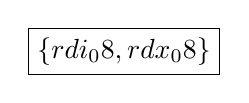
\begin{tikzpicture}[>=stealth, every node/.style={draw}]
      \node (a) {$\{\region{\reg{rdi}_0}{8},\region{\reg{rdx}_0}{8}\}$};
    \end{tikzpicture}%
    \hspace{3ex}
  }
  \hfill
  \subcaptionbox{Join result\label{fig:otherMemJoin}}{
    \hspace{2ex}
    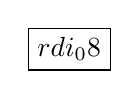
\begin{tikzpicture}[>=stealth, every node/.style={draw}]
      \node (a) {$\region{\reg{rdi}_0}{8}$};
    \end{tikzpicture}%
    \hspace{2ex}
  }
  \hspace*\fill
  \caption{Join with alternate memory model}\label{fig:otherJoin}
  %\Description{This shows an alternate memory model (on the left,
    %containing two eight-byte regions with separate symbolic variable bases)
    %that is joined with the memory model from Figure~\ref{fig:memA}
    %(where one of the top-level regions is shared),
    %resulting in the memory model shown on the right in the figure.
    %(only that shared top-level region is present)}
\end{figure}

\begin{example}
  \todo{figure out if this and the related figure should be included}
  First, consider the memory models shown in \cref{fig:mem}.
  Since the top nodes share a region, the two trees belong to the same equivalence class.
  The intersection of all of the region alias sets is:
  \begin{equation*}
    \{\region{\reg{rdi}_0}{8},\region{\reg{rsi}_0}{8}\}\cap
    \{\region{\reg{rdi}_0}{8}\}\cap\{\region{\reg{rsi}_0}{8}\}
  \end{equation*}
  As this intersection produces $\varnothing$,
  the result of the join is $\varnothing$, an empty memory model.
  Second, the join of the memory model shown in \cref{fig:memA}
  with the one shown in \cref{fig:otherMem} results in the memory model shown in \cref{fig:otherMemJoin}.
  This is because all top-level memory trees involved in the merge share
  a region, $\region{\reg{rdi}_0}{8}$, but have no comparable children.
\end{example}

We prove that the join over memory models is sound.
\begin{lemma}\label{lem:mem_soundness}
  Let~$s$ be a state and~$M_0$ and~$M_1$ be memory models. Then:
  \begin{equation*}
    (s\models M_0 \vee M_1) \implies (s\models M_0\sqcup M_1)
  \end{equation*}
\end{lemma}
\begin{proof}
  Let $r_0\mathbin{\square}r_1$ be a relation in $\mathcal{R}(M_0 \sqcup M_1)$.
  If $\square$ is $\equiv$, then both regions $r_0$ and $r_1$ must have been present in all trees in the corresponding equivalence class.
  The relation thus held in either $M_0$ or $M_1$.
  If $\square$ is $\bowtie$, then the two regions are from trees generated from different equivalence classes. Since they are from trees that do not share a top-level region, the original trees in either $M_0$ or $M_1$ are separate as well.
  Similar reasoning applies for the other cases.
\end{proof}


\begin{definition}
  The join of some two symbolic states $\sigma_0=\langle P_0,M_0\rangle$
  and $\sigma_1=\langle P_1,M_1\rangle$, notation $\sigma_0 \sqcup \sigma_1$, is:
  \begin{equation*}
    \sigma_0 \sqcup \sigma_1 \defeq \langle P_0\sqcup P_1,M_0\sqcup M_1\rangle
  \end{equation*}
\end{definition}

We would like to remark that this join loses information.
It can thus only be applied in a sound fashion for postcondition weakening \autocite{hoare1969axiomatic}.
In other words, dropping clauses and performing state cleanup
serve only to reduce state constraints; they never add additional ones.
In practice, this loss of information means that we may produce a state
that would not actually be encountered during program execution,
or we may be unable to resolve some indirections/prove some return addresses
(which would result in annotations/tool failure).
Even in such cases, given successful completion and no annotations produced,
we will always produce all states that would be encountered during concrete execution.

\section{Base Algorithm}
\todo{maybe move this to Technical Formulation?}
\Ac{hg}

\section{Extension: Function Calls}

\subsection{External Functions}

\subsection{Internal Functions}
